\documentclass[../../main.tex]{subfiles}
% \documentclass[a4paper,10pt]{ltjsarticle}
\begin{document}
\rhead{京都大学後期$1998$年$5$番}
\setcounter{equation}{0}
\begin{oframed}
  \documentclass[../../main.tex]{subfiles}
\begin{document}

$xy$平面上に$2n$個の点$\mathrm{A}_i(i,1)$，$\mathrm{B}_i(i,2) (i=1,2,\cdots,n)$がある．
上下に隣り合う$2$点$\mathrm{A}_i$，$\mathrm{B}_i$を結ぶ線分を「縦辺」$(i=1,2,\cdots,n)$，左右に隣り合う$2$点$\mathrm{A}_i$，$\mathrm{A}_{i+1}$および$\mathrm{B}_i$，$\mathrm{B}_{i+1}$を結ぶ線分を「横辺」$(i=1,2,\cdots,n-1)$と言う．
全ての横辺には，各辺独立に，確率$p$で右向きの矢印が，確率$1-p$で$\times$印が描かれている．
また全ての縦辺には常に上向きの矢印が描かれている．
このとき点$\mathrm{A}_1(1,1)$から出発して，矢印の描かれている辺だけを通り，矢印の方向に進んで，点$\mathrm{B}_{n}(n,2)$に到達する経路が少なくとも$1$本存在する確率を$Q_n$とする．
以下の問に答えよ．
\begin{enumerate}
  \item $Q_2$，$Q_3$を求めよ．
  \item $Q_n$を求めよ．
\end{enumerate}

\end{document}

\end{oframed}
\setlength{\columnseprule}{0.4pt}
\begin{multicols}{2}
  {\bf [解答]}

  まず，明らかに
  \begin{align}
    Q_1 = 1
  \end{align}
  である．$A_i,B_i$を図示すると\cref{1998-5:fig:1}のようになる．

  \begin{figure}[H]
    \centering
    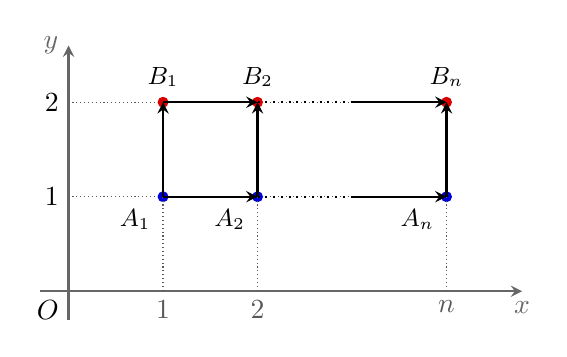
\begin{tikzpicture}[x=1.2cm, y=1.2cm, >=stealth]
      % Coordinate axes
      \draw[->, thick, gray!80!black] (-0.3,0) -- (4.8,0) node[below] {$x$};
      \draw[->, thick, gray!80!black] (0,-0.3) -- (0,2.6) node[left] {$y$};

      % Labels for coordinates on axes
      \node[below left] at (0,0) {$O$};
      \node[left] at (0,1) {$1$};
      \node[left] at (0,2) {$2$};
      \draw[densely dotted, gray!70!black] (0,1) -- (4,1);
      \draw[densely dotted, gray!70!black] (0,2) -- (4,2);

      % Points A on y=1
      \coordinate (A1) at (1,1);
      \coordinate (A2) at (2,1);
      \coordinate (An) at (4,1);
      \node[circle, fill=blue!85!black, inner sep=1.4pt] at (A1) {};
      \node[circle, fill=blue!85!black, inner sep=1.4pt] at (A2) {};
      \node[circle, fill=blue!85!black, inner sep=1.4pt] at (An) {};
      \node[below left=1pt, font=\small] at (A1) {$A_1$};
      \node[below left=1pt, font=\small] at (A2) {$A_2$};
      \node[below left=1pt, font=\small] at (An) {$A_n$};

      % Points B on y=2
      \coordinate (B1) at (1,2);
      \coordinate (B2) at (2,2);
      \coordinate (Bn) at (4,2);
      \node[circle, fill=red!85!black, inner sep=1.4pt] at (B1) {};
      \node[circle, fill=red!85!black, inner sep=1.4pt] at (B2) {};
      \node[circle, fill=red!85!black, inner sep=1.4pt] at (Bn) {};
      \node[above=2pt, font=\small] at (B1) {$B_1$};
      \node[above=2pt, font=\small] at (B2) {$B_2$};
      \node[above=2pt, font=\small] at (Bn) {$B_n$};

      % Ticks and projections to x-axis
      \draw[densely dotted, gray!70!black] (A1) -- (1,0) node[below] {$1$};
      \draw[densely dotted, gray!70!black] (A2) -- (2,0) node[below] {$2$};
      \draw[densely dotted, gray!70!black] (An) -- (4,0) node[below] {$n$};

      % Horizontal arrows for A
      \draw[->, thick] (A1) -- (A2);
      \draw[dotted, thick] (A2) -- (3,1);
      \draw[->, thick] (3,1) -- (An);

      % Horizontal arrows for B
      \draw[->, thick] (B1) -- (B2);
      \draw[dotted, thick] (B2) -- (3,2);
      \draw[->, thick] (3,2) -- (Bn);

      % Vertical arrows A to B
      \draw[->, thick] (A1) -- (B1);
      \draw[->, thick] (A2) -- (B2);
      \draw[->, thick] (An) -- (Bn);
    \end{tikzpicture}
    \caption{$A_i,B_i$の様子}
    \label{1998-5:fig:1}
  \end{figure}

  \paragraph{(1)}
  \textbf{$n=2$ の時}

  \begin{figure}[H]
    \centering
    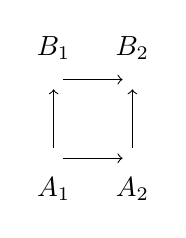
\begin{tikzpicture}
      % Points A
      \node[label=below:$A_1$] (A1) at (0,0) {};
      \node[label=below:$A_2$] (A2) at (1,0) {};

      % Points B
      \node[label=above:$B_1$] (B1) at (0,1) {};
      \node[label=above:$B_2$] (B2) at (1,1) {};

      % Arrows
      \draw[->] (A1) -- (A2);
      \draw[->] (B1) -- (B2);
      \draw[->] (A1) -- (B1);
      \draw[->] (A2) -- (B2);
    \end{tikzpicture}
    \caption{$n=2$の時の様子}
    \label{1998-5:fig:2}
  \end{figure}

  $A_1 \to A_2 \to B_2$, 又は $A_1 \to B_1 \to B_2$ と行けば良い．
  排反事象を考えると，これは$A_1A_2$にも$B_1B_2$にも×がついている時以外である．
  従って，求める確率は
  \begin{align}
    Q_2 & = 1 - (1-p)^2 \\
    & = p(2-p)
  \end{align}
  である．$\cdots$(答)
  \vspace{10pt}

  \textbf{$n=3$ の時}

  \begin{figure}[H]
    \centering
    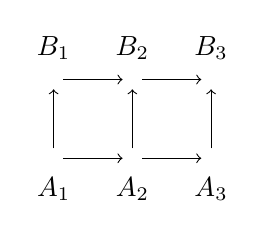
\begin{tikzpicture}
      % Points A
      \node[label=below:$A_1$] (A1) at (0,0) {};
      \node[label=below:$A_2$] (A2) at (1,0) {};
      \node[label=below:$A_3$] (A3) at (2,0) {};

      % Points B
      \node[label=above:$B_1$] (B1) at (0,1) {};
      \node[label=above:$B_2$] (B2) at (1,1) {};
      \node[label=above:$B_3$] (B3) at (2,1) {};

      % Arrows
      \draw[->] (A1) -- (A2);
      \draw[->] (A2) -- (A3);
      \draw[->] (B1) -- (B2);
      \draw[->] (B2) -- (B3);
      \draw[->] (A1) -- (B1);
      \draw[->] (A2) -- (B2);
      \draw[->] (A3) -- (B3);
    \end{tikzpicture}
    \caption{$n=3$の時の様子}
    \label{1998-5:fig:3}
  \end{figure}

  $A_1$ から右方向へ出発し，どこではじめて上方へ移動しなければならないか
  ($A_k A_{k+1}$ が $\times$ となっている最小の$k \in \mathbb{N}$) で場合分けする．
  \begin{enumerate}
    \item $A_1 A_2$ が $\times$ の時，$A_1 \to B_1$ へ行くルートで確率は $p^2 (1-p)$
    \item $A_2 A_3$ が $\times$ の時，$B_2 B_3$ が矢印になっていれば良く，確率は $p^2 (1-p)$
    \item $A_1 A_2, A_2 A_3$ とも通過できる時，必ずルートがあって確率は $p^2$
  \end{enumerate}
  以上三つの場合は互いに排反だから，求める確率は
  \begin{align}
    Q_3
    & = 2p^2 (1-p) + p^2 \\
    & = p^2 (3-2p)
  \end{align}
  である．$\cdots$(答)
  \vspace{10pt}

  \paragraph{(2)}

  (1)の $n=3$ の時と同様の場合分けをする．
  つまり，$A_1$ から右へ進んでいって，はじめて行き止まり ($\times$) になっている所が
  $A_k A_{k+1}$ の時を考える($k=1, 2, \dots, n-1$)．
  (以下 $n \ge 4$ とする．

    この時．$B_n$ まで行ける確率は $C_n(k)$ とおく．
    この確率は$A_1 \to \dots \to A_k$まで行き，そのあと$B_k \to \dots \to B_n$
    が行き止まりになっておらず矢印になっており，$A_k A_{k+1}$ が $X$ になっている時で，
    \begin{align}
      a_n(k) = p^{n-1} \cdot (1-p)
    \end{align}
    である．

    また，Aの横道に一つも行き止まりがない時を便宜上$k=n$とおくと
    \begin{align}
      a_n(n) = p^{n-1}
    \end{align}
    である．

    従って，各$a_{n}(k)$は排反事象であることより，求める確率は
    \begin{align}
      Q_n
      & = \sum_{k=1}^{n} a_n(k)            \\
      & = \sum_{k=1}^{n-1} a_n(k) + a_n(n) \\
      & = (n-1) p^{n-1} (1-p) + p^{n-1}     \\
      & = p^{n-1} \{ n - (n-1)p \}
    \end{align}
    である．(1)より，これは$n=2,3$ でも成立するから，求める確率は
    \begin{align}
      Q_n = p^{n-1} \{ n - (n-1)p \}
    \end{align}
    である．$\cdots$(答)

    \vspace{10pt}
    {\bf [解説]}

    % TODO :: 漸化式を立てる方法も有力
    % 下側にたどり着く確率$alpha_i$，上側にたどり着く確率$beta_i$とすると
    % \alpha_{n+1} = p\alpha_{n}

    % \beta_{n+1} = p\beta_{n} + p(1-p)\alpha_n
    % であり，これは解ける．
    \newpage

  \end{multicols}
  \end{document}
